\section{Atmosphere}
\label{sec:atmosphere}

\subsection{Extinction}

Zenith transmission $T_{\rm atm}(\lambda)$ comes either from a
site-specific FITS table (e.g.\ the Paranal product, whose
\code{EXTINCTION} column in mag\,airmass$^{-1}$ is converted once as
$T=10^{-0.4k_\lambda}$) or from the built-in broad-band $U$--$K$ table
(Table~\ref{tab:sky}). The Bouguer law applies it as $T^{X}$, exactly once,
to the source; observed sky brightnesses are never extinguished a second
time.

\subsection{Refraction and airmass}
\label{sec:airmass}

Apparent altitudes include ERFA atmospheric refraction evaluated at the
ISA pressure and temperature of the site elevation,
$P = \SI{1013.25}{hPa}\,e^{-E/\SI{8435}{m}}$ and
$T = \SI{15}{\celsius} - 0.0065\,E$. The airmass is the
\citet{pickering2002} interpolative formula on the \emph{apparent} altitude
$h$ (degrees),
\begin{equation}
  X \;=\; \frac{1}{\sin\!\big(h + 244/(165 + 47\,h^{1.1})\big)},
  \label{eq:pickering}
\end{equation}
which matches $\sec z$ near the zenith and remains physical to the horizon,
where the plane-parallel form diverges (Fig.~\ref{fig:airmass}). The ETC
deliberately reports no airmass below $h=5^\circ$.

\begin{figure}
  \centering
  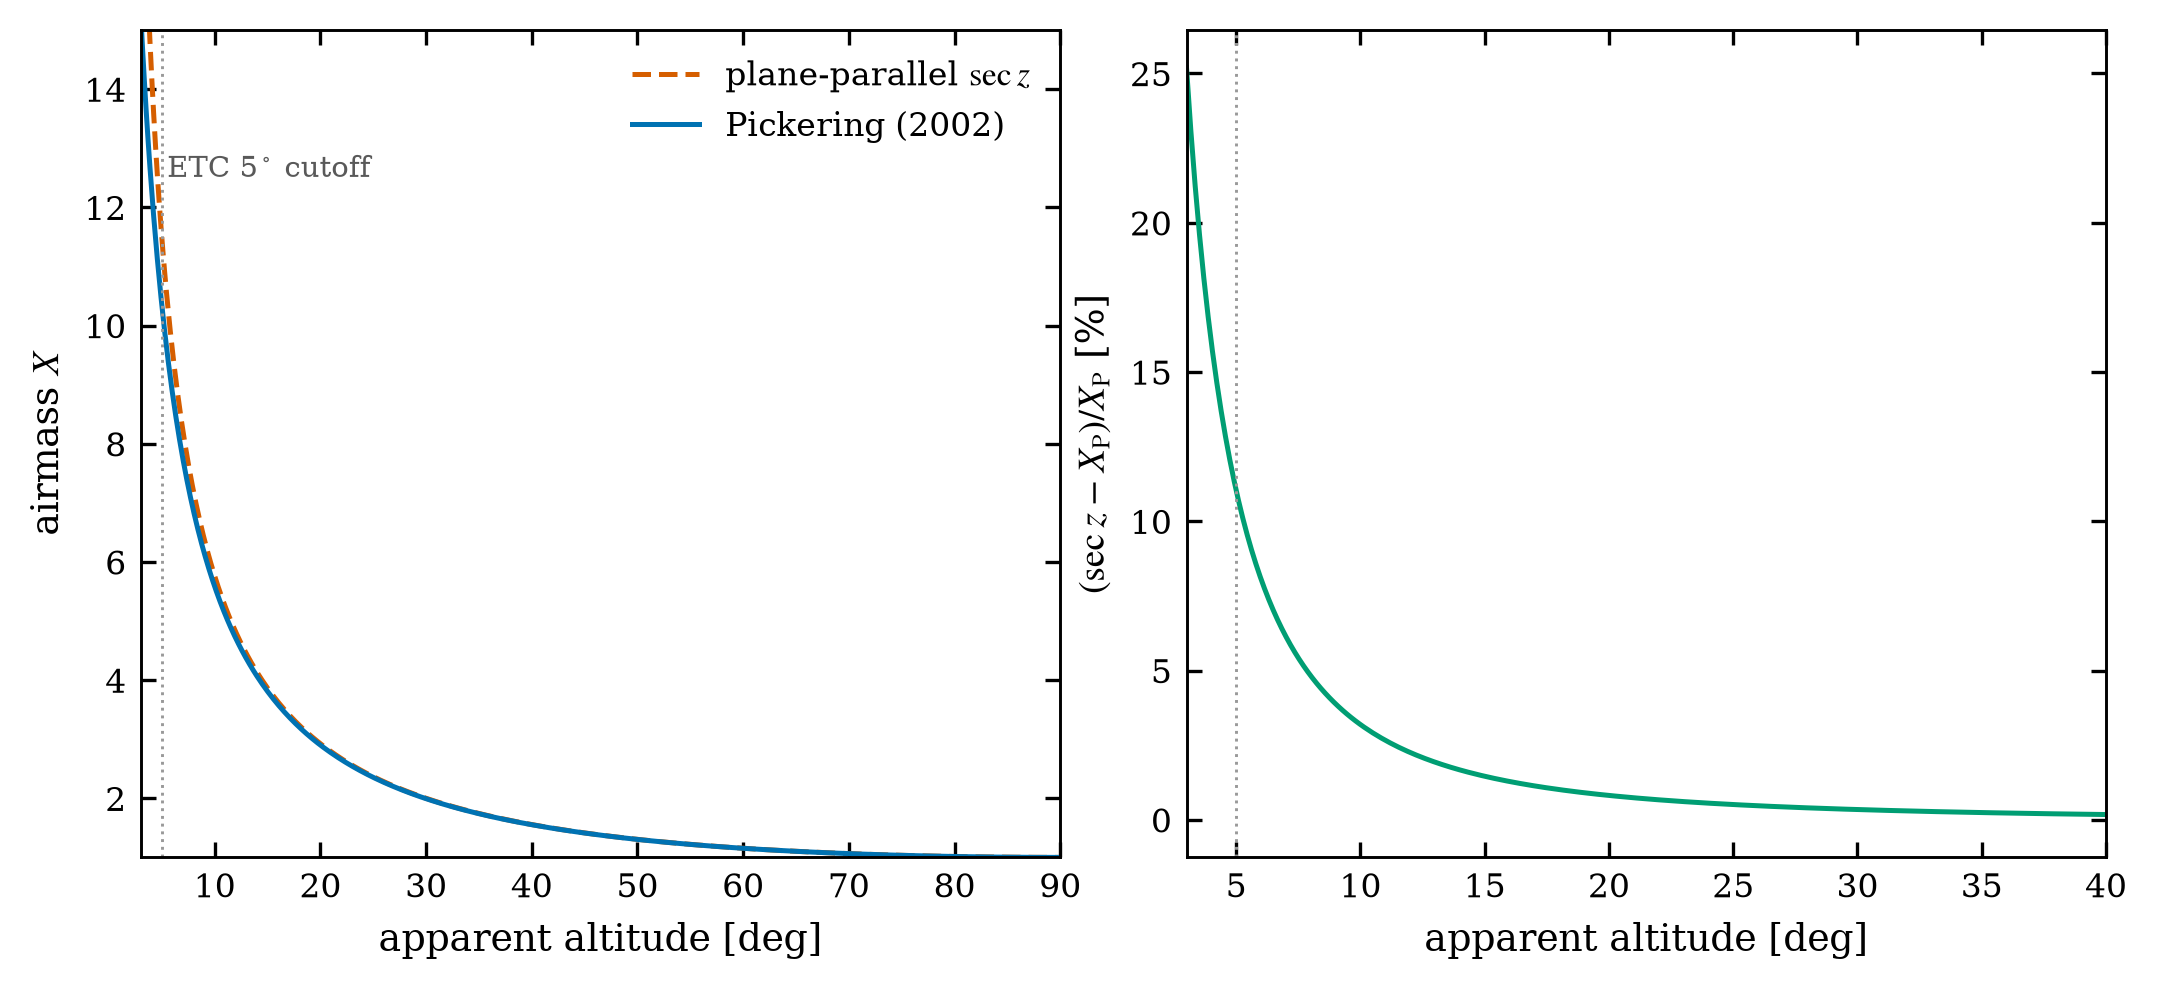
\includegraphics[width=\textwidth]{figures/fig_02_airmass.png}
  \caption{Left: Pickering (2002) airmass versus plane-parallel $\sec z$.
  Right: relative overestimate of $\sec z$; at the ETC's $5^\circ$ cutoff it
  already exceeds 10\%.}
  \label{fig:airmass}
\end{figure}

\subsection{Differential atmospheric refraction}
\label{sec:dispersion}

The refractive index of air follows \citet{filippenko1982}: at standard
conditions
\begin{equation}
  (n-1)\,10^{6} = 64.328 + \frac{29498.1}{146-\sigma^2}
                 + \frac{255.4}{41-\sigma^2},\qquad \sigma = 1/\lambda_{\mu m},
\end{equation}
rescaled to the site pressure and temperature with his equations (2)--(3),
including the water-vapour term. The differential refraction relative to a
reference wavelength is
\begin{equation}
  \Delta R(\lambda) = 206265\,\big[n(\lambda)-n(\lambda_{\rm ref})\big]\tan z ,
  \label{eq:dr}
\end{equation}
about $1''$ between 4000 and \SI{5500}{\angstrom} at $z=45^\circ$
(Fig.~\ref{fig:dispersion}). Its use in slit losses is described in
Sect.~\ref{sec:slit}; the parallactic angle
\begin{equation}
  q \;=\; \arctan\!\frac{\sin H}{\tan\varphi\cos\delta - \sin\delta\cos H}
  \label{eq:parallactic}
\end{equation}
($H$ hour angle, $\varphi$ latitude, $\delta$ declination) is reported for
every time sample, because a slit oriented at $q$ suffers no dispersion
loss.

\begin{figure}
  \centering
  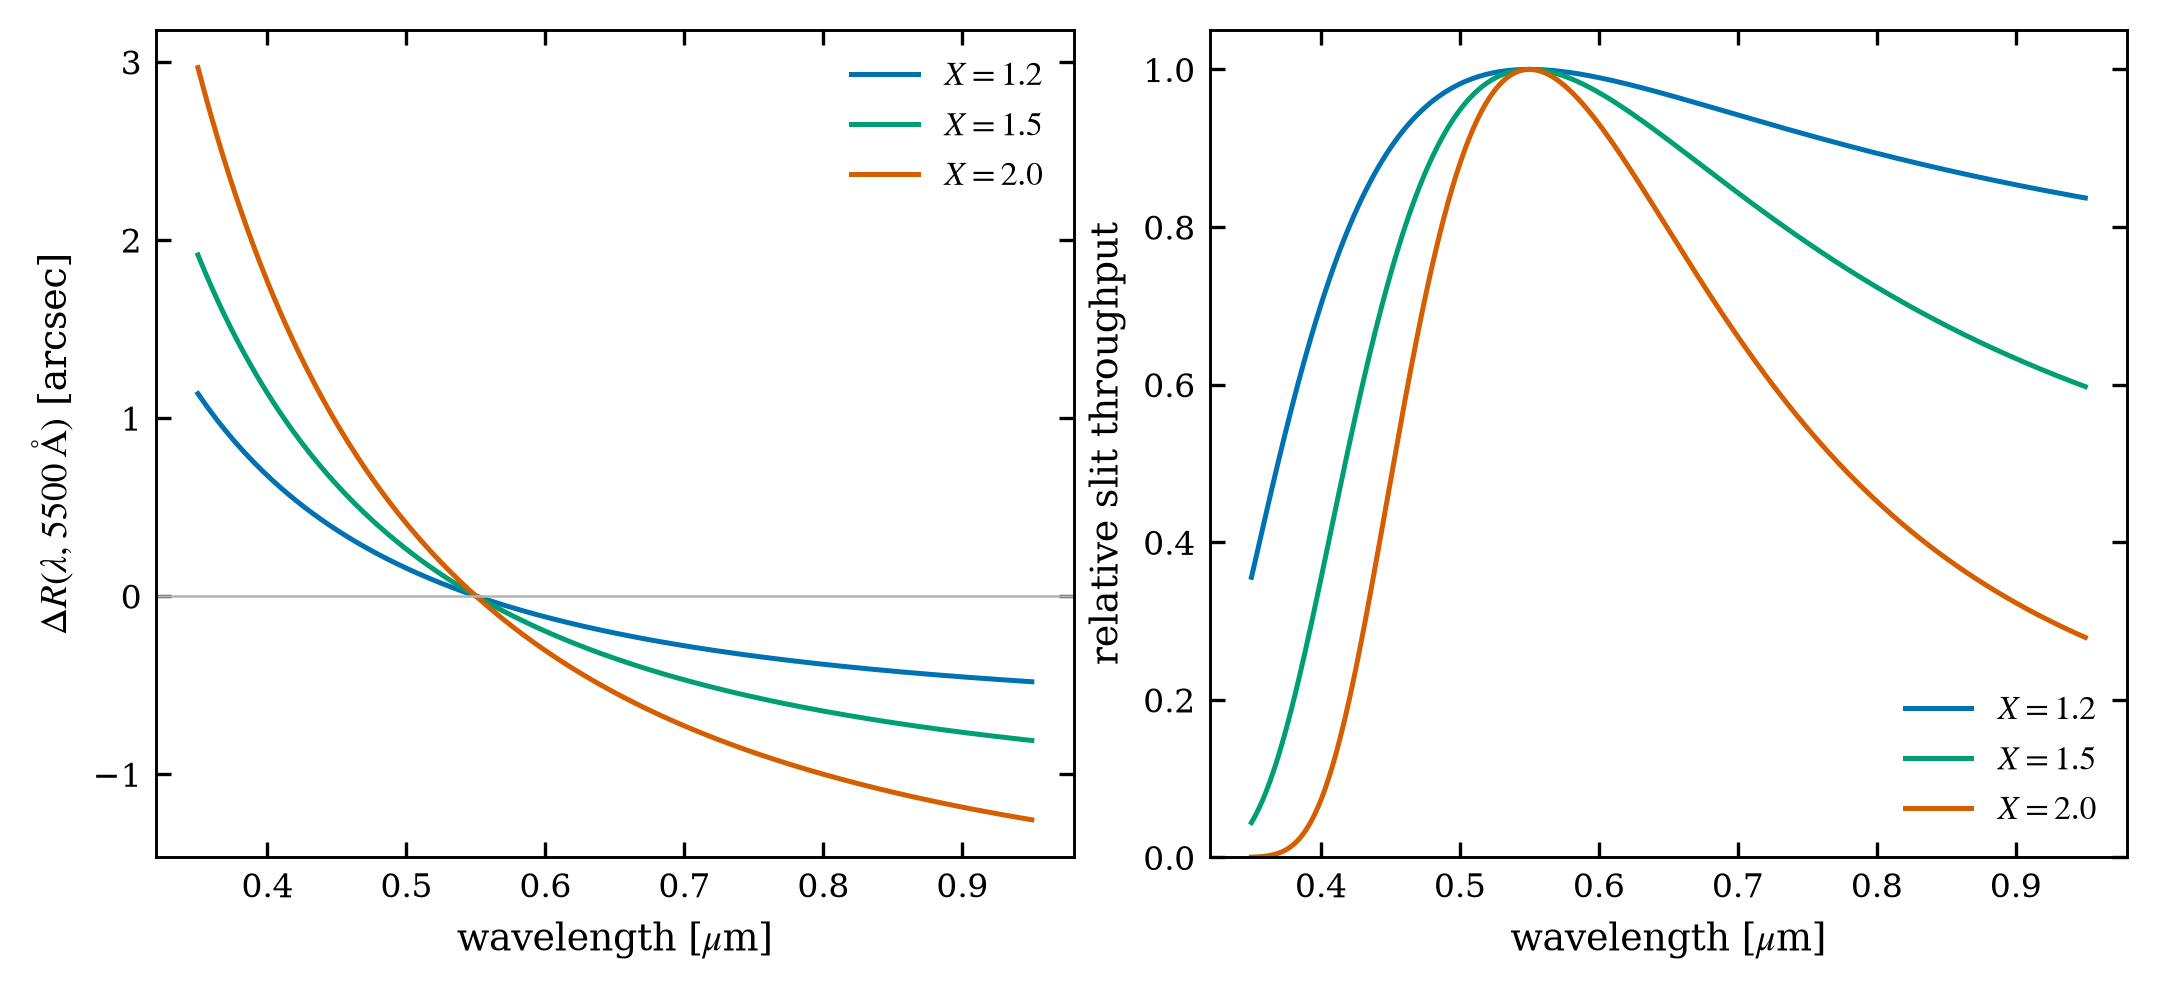
\includegraphics[width=\textwidth]{figures/fig_05_dispersion.png}
  \caption{Left: differential refraction relative to \SI{5500}{\angstrom}
  for three airmasses. Right: resulting relative slit throughput for a
  $1.5''$ slit in $1.5''$ seeing when the slit is \emph{not} at the
  parallactic angle (worst-case geometry).}
  \label{fig:dispersion}
\end{figure}

\subsection{Scintillation}
\label{sec:scintillation}

Intensity scintillation follows the \citet{young1967} law, kept in the
functional form endorsed by \citet{osborn2015},
\begin{equation}
  \frac{\sigma_{\rm scint}}{I} \;=\;
  0.09\; d_{\rm cm}^{-2/3}\, X^{1.75}\,
  e^{-E/\SI{8000}{m}}\,(2\,t_{\rm exp})^{-1/2},
  \label{eq:scint}
\end{equation}
with $d$ the aperture diameter, $E$ the site elevation and $t_{\rm exp}$
the exposure time. Because this noise is multiplicative in the source flux,
it dominates bright-star photometry and imposes a hard S/N ceiling
$\simeq I/\sigma_{\rm scint}$ per exposure (Fig.~\ref{fig:snrbudget}).
